\section{Exercise 2}\label{sect: P2E2}
Here we are asked to make a Brownian simulation with a WCA potential of which the code will be found in appendix~\ref{app:P2E2}.
The Weeks Chandler Andersen (WCA) potential is a modified Lennard Jones potential that is cut of at the minimum of the original Lennard Jones potential 
and shifted up to 0 at the minimum to create a purely repulsive potential:

\begin{align}
V(r) = \begin{dcases} 4 \epsilon \left[\left( \frac{\sigma}{r} \right)^{12} - \left( \frac{\sigma}{r} \right)^6\right] + \epsilon &,r \le  r_0 \\ 0  &,r > r_0. \end{dcases}
\end{align}\label{eq: WCA potential}

Where $r_0 = 2^{\frac{1}{6}} \sigma$ is the minimum of the Lennard Jones potential. And therefore we get the following force:
\begin{align}
F_{WCA}(r) = - \nabla V(r) = \begin{dcases} \frac{48 \epsilon}{r} \left[ \left(\ \frac{\sigma}{r}\right)^{12}-\frac{1}{2}\left(\frac{\sigma}{r}\right)^6\right]   &,r \le  r_0 \\ 0  &,r > r_0. \end{dcases}
\end{align}\label{eq: WCA force}
This is the same force as in the Lennard Jones potential up to minima at $r_0$.

For Brownian motion we get the following integration scheme:

\begin{align}
    x(t +\Delta t) = x(t) + \sqrt{2D}R(t)\sqrt{\Delta t} + \frac{F^x_{int}}{\gamma} \Delta t.
\end{align}\label{eq: brownian integration}

Here $D = \frac{k_BT}{\gamma}$ is the diffusion constant, $\gamma$ is the friction constant, $R(t)$ is the random Brownian force characterized by $\left\langle R(t)\right\rangle = 0,\quad \left\langle R_i(t)R_j(t')\right\rangle = \delta(t-t')\delta_{ij}$
and $F^x_{int}$ is the resulting interaction force coming from the WCA potential in our case.

\subsection{Energy vs time step}
Using the integration from equation \ref{eq: brownian integration} starting from an FCC lattice at a density of $\rho \sigma^3 = 0.5$ and a temperature of $\frac{k_B T}{\epsilon} = 1$ we get:
\begin{figure}[H]
	\centering
	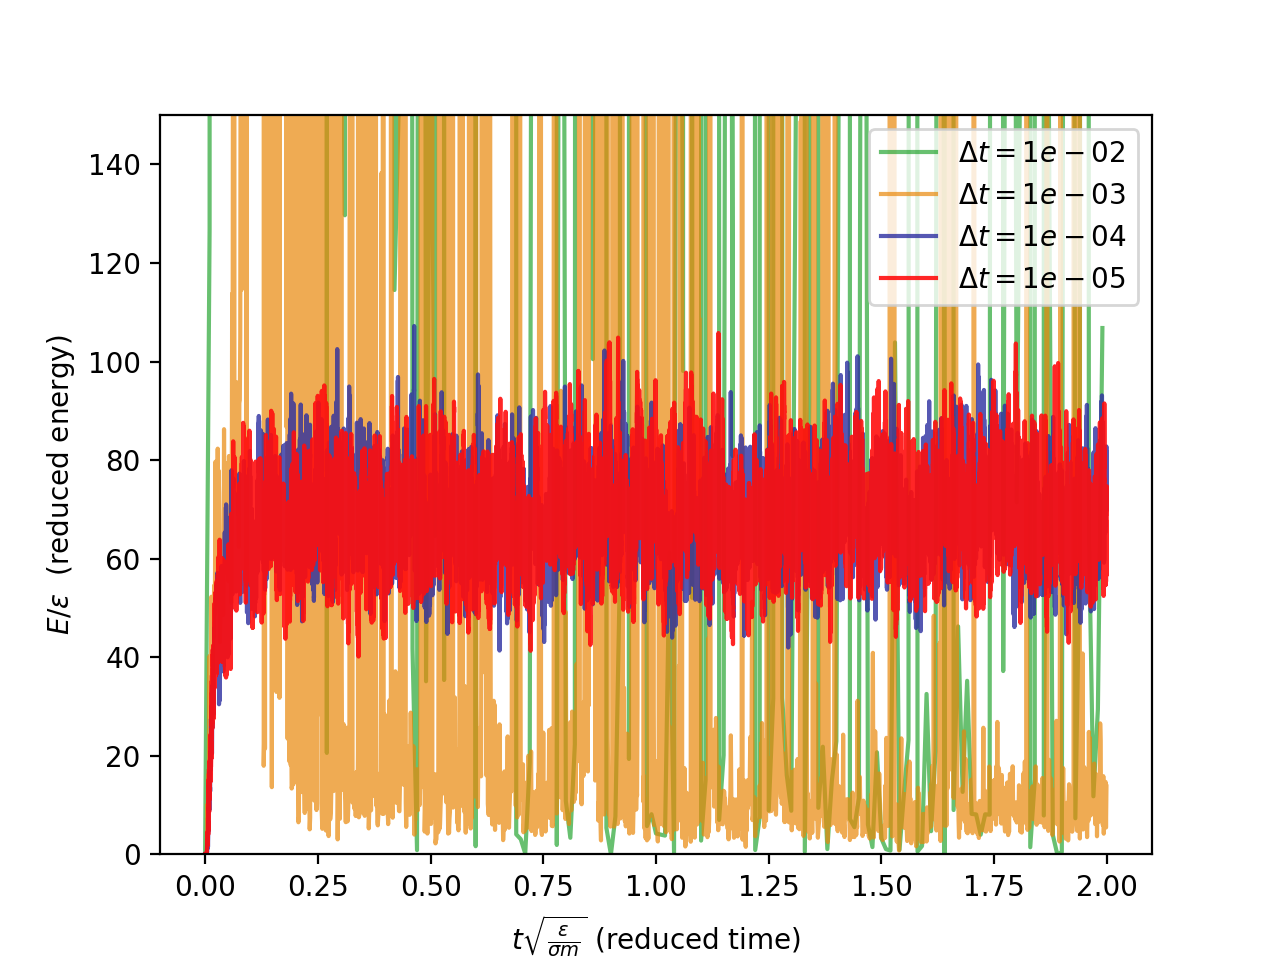
\includegraphics[width=0.75\linewidth]{graphs/P2E2/energy_vs_dt.png}
	\caption{Reduced energy versus reduced time for 4 different time steps.}
	\label{fig: energy vs dt}
\end{figure}
We notice that the energy first equilibrates and then oscillates around an average value for time steps smaller than $\Delta t = 10^{-4}$ and becomes unstable for larger timesteps.
Therefore, the largest stable time step $\Delta t = 10^{-4}$ is a good time step.

\newpage
\subsection{Energy vs temperature}
For this section we continue with the time step of $\Delta t = 10^{-4}$ for all temperatures and use a constant density of $\rho \sigma^3 = 0.5$.
For these parameters we get the following energies:
\begin{figure}[H]
	\centering
	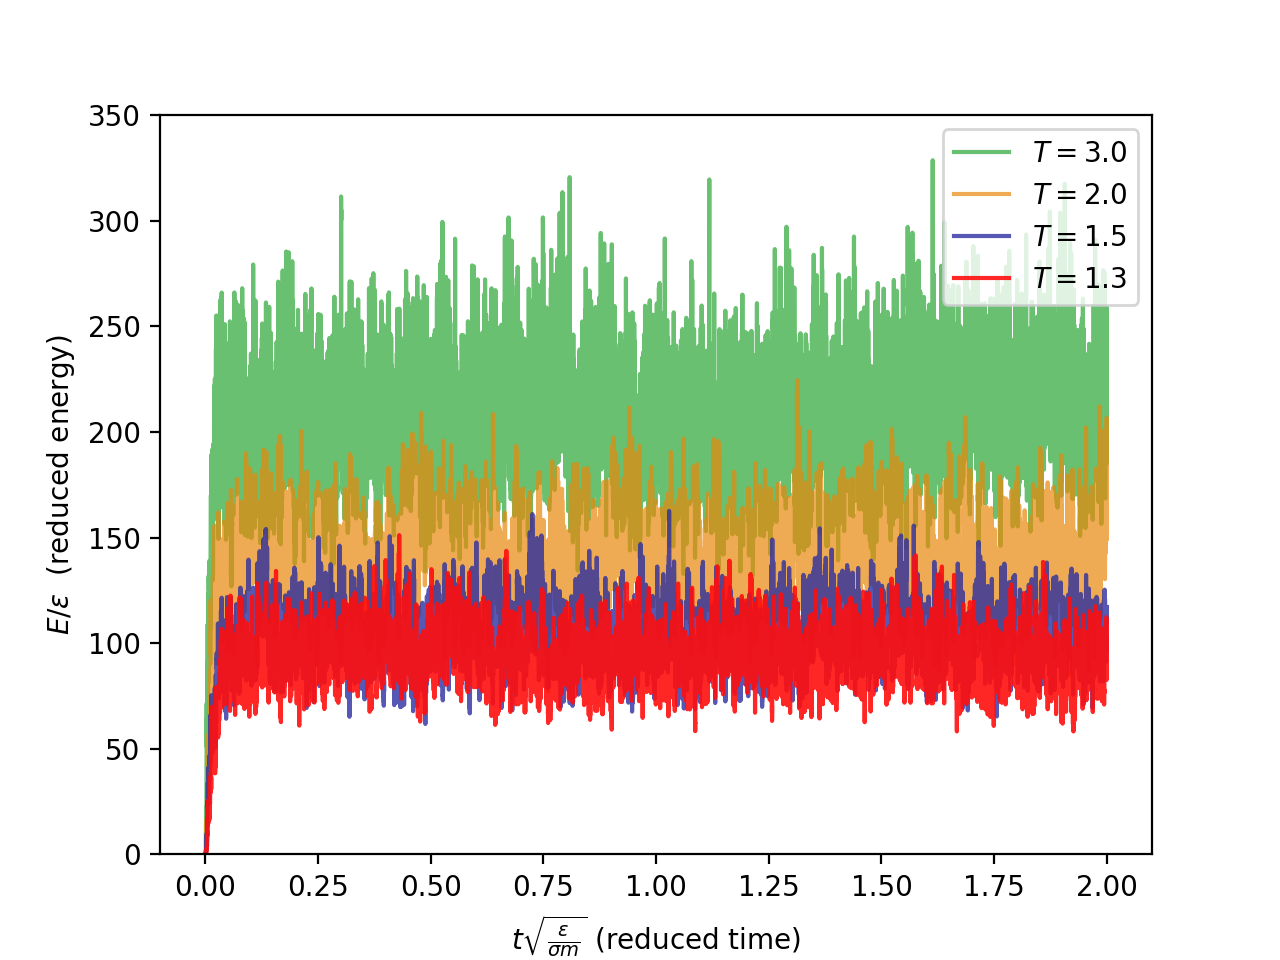
\includegraphics[width=0.7\linewidth]{graphs/P2E2/energy_vs_T.png}
	\caption{Reduced energy versus reduced time for 4 different temperatures.}
	\label{fig: energy vs T}
\end{figure}
We see a general trend across all temperatures where the energy first increase and then oscillates around an average value.
For higher temperatures we see a higher average temperature and a bigger oscillation around the average. \\
To look at the equilibration time we use the Savitzky-Golay filter to smooth the energy. 
We see that across all temperatures the energy equilibrates after a reduced time of about 0.1.
\begin{figure}[H]
	\centering
	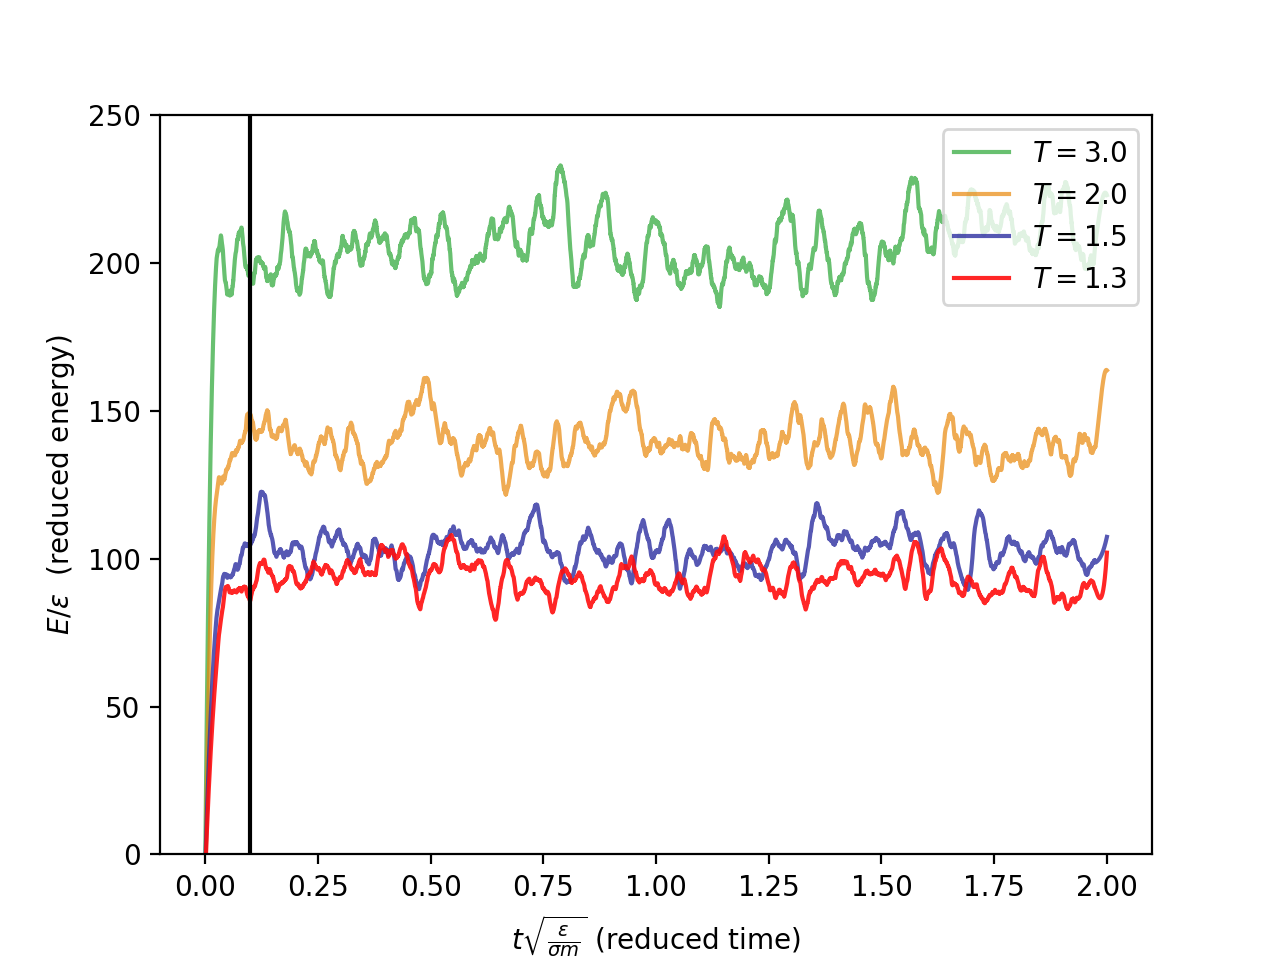
\includegraphics[width=0.7\linewidth]{graphs/P2E2/smooth_energy_vs_T.png}
	\caption{Reduced smoothed energy using the Savitzky-Golay filter versus reduced time for 4 different temperatures. The vertical line is at a reduced time of 0.1 and indicate the equilibration time }
	\label{fig:smooth energy vs T}
\end{figure}

\newpage
\subsection{MSD for $\bf{\rho \sigma^3 = 0.01}$}
For our choice of  $\Delta t$ and $\rho$ we get the following MSD:
\begin{figure}[H]
	\centering
	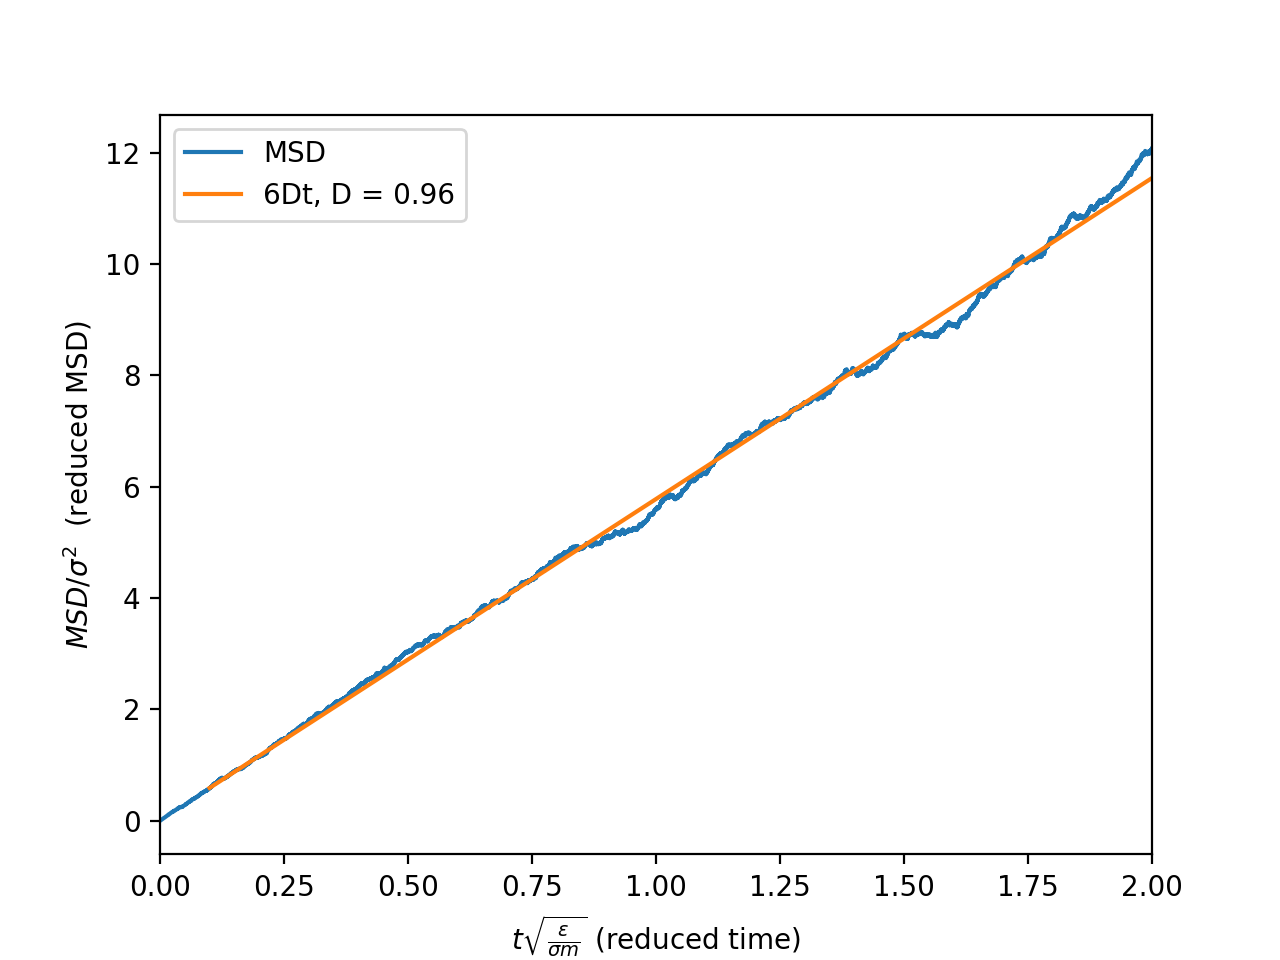
\includegraphics[width=0.7\linewidth]{graphs/P2E2/MSD.png}
	\caption{MSD displacement with linear fit for $\rho \sigma^3 = 0.01$. }
	\label{fig: MSD}
\end{figure}
Here we have plotted a linear fit of 6Dt where we have taken the fit after the equilibrium time of 0.1. 
We find a diffusion constant of 0.96. We see that the data follows the linear fit form the theoretical model of 6Dt well.

\subsection{MSD for $\bf{\rho \sigma^3 = 0.6}$}
For the higher density we get the following MSD:
\begin{figure}[H]
	\centering
	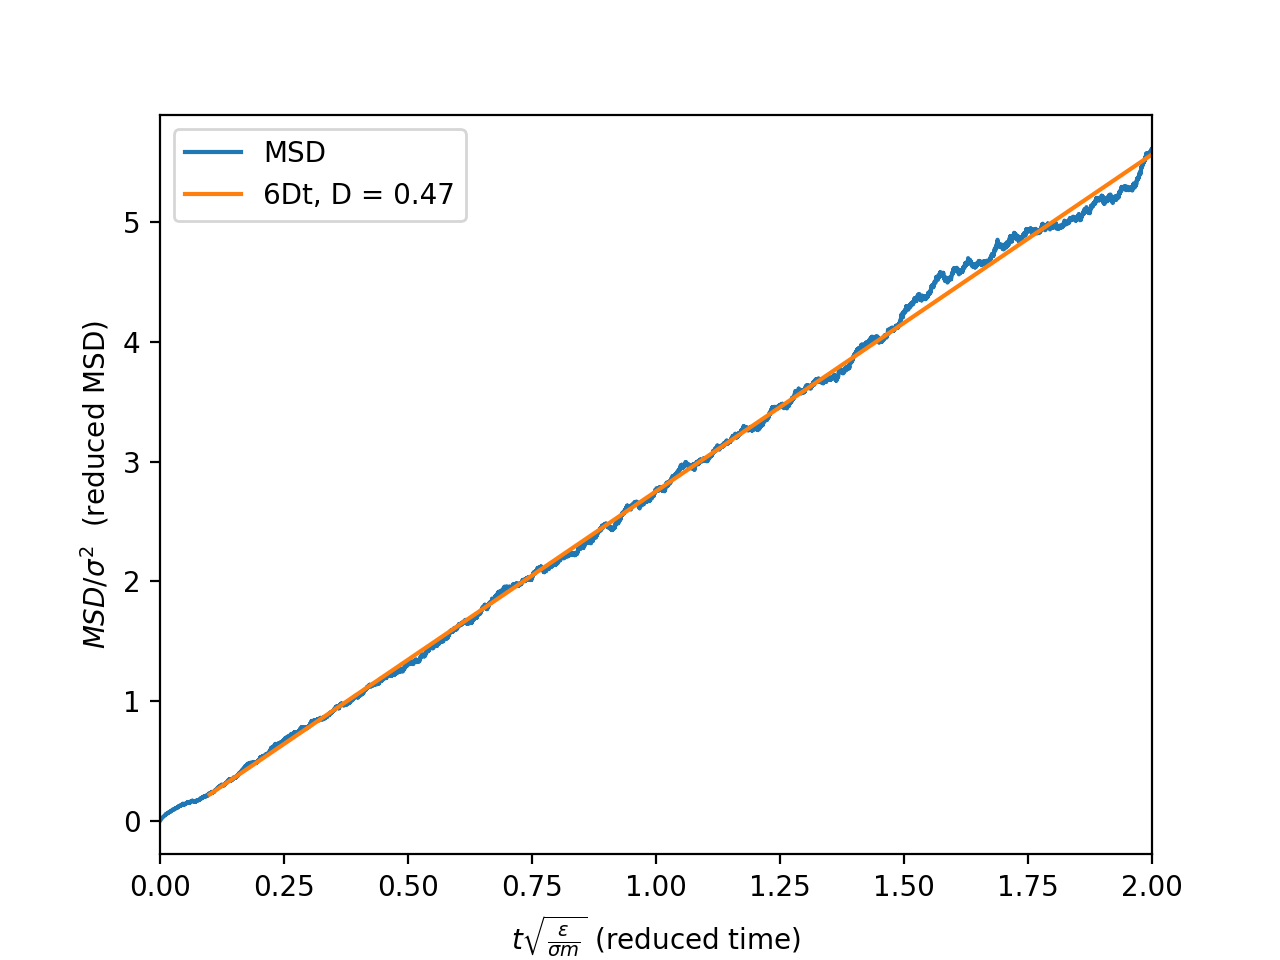
\includegraphics[width=0.7\linewidth]{graphs/P2E2/MSD_0.6.png}
	\caption{MSD displacement with linear fit for $\rho \sigma^3 = 0.6$.}
	\label{fig: MSD 0.6}
\end{figure}
We see that the data again matches the theoretical linear model well but this time with a lower diffusion constant of 0.47 which is to be expected for a higher density.

\newpage
\subsection{MSD for $\bf{\rho \sigma^3 = 1.15}$}
For our last and highest density starting in an FCC latice we get the following MSD:
\begin{figure}[H]
	\centering
	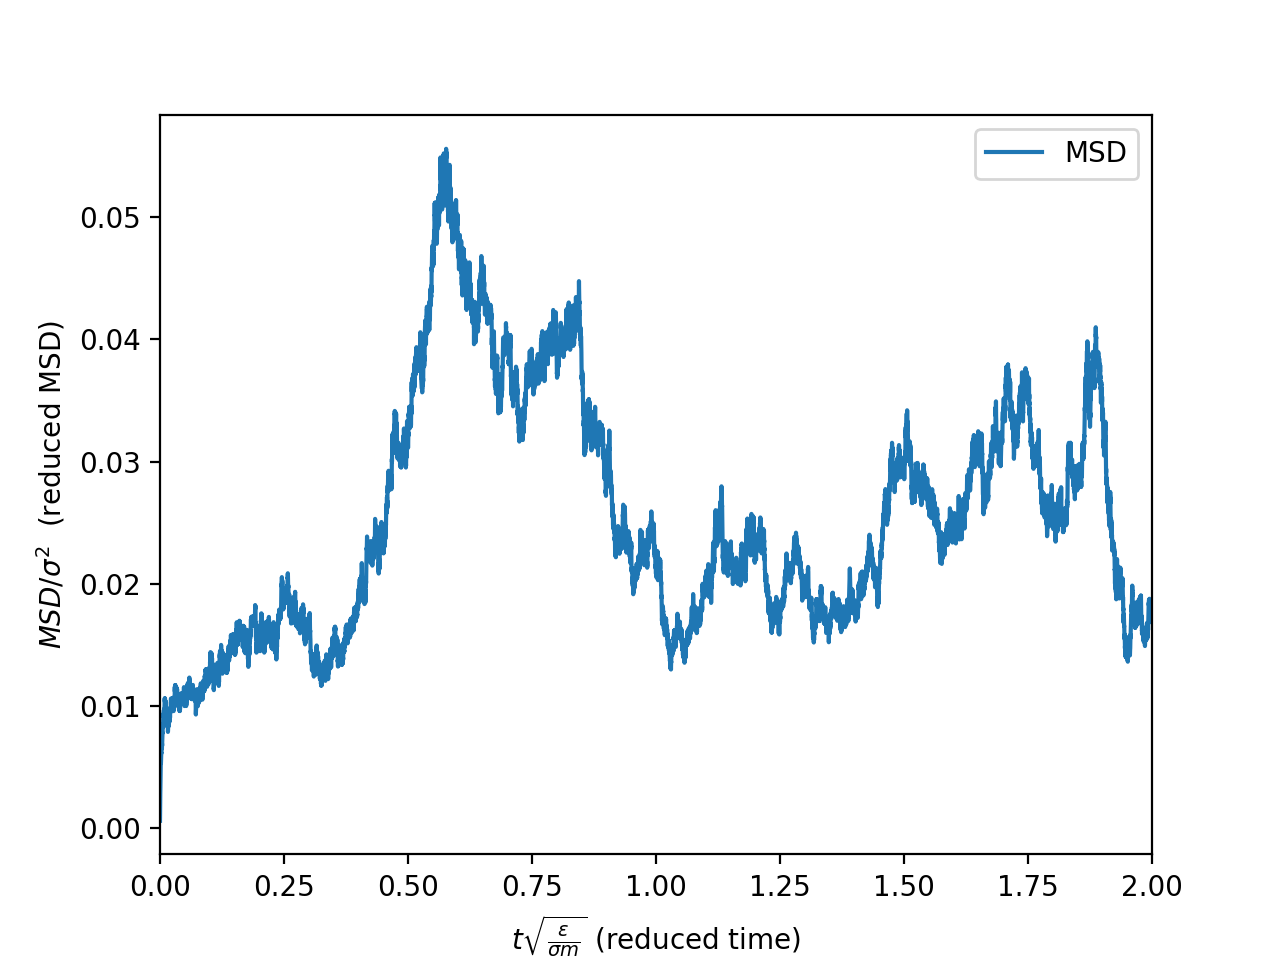
\includegraphics[width=0.7\linewidth]{graphs/P2E2/MSD_1.15.png}
	\caption{MSD displacement with linear fit for $\rho \sigma^3 = 1.15$.}
	\label{fig: MSD 1.15}
\end{figure}
For our highest density we see a drastically different MSD. We see no linear increasing trend but rather a stochastic MSD.
This is because of a phase transition. The particles are now in a solid phase and not free to move creating this stochastic movement in the FCC lattice.\\
We also see this in the final coordinates where we see the particles are still inside an FCC lattice.

\begin{figure}[H]
	\centering
	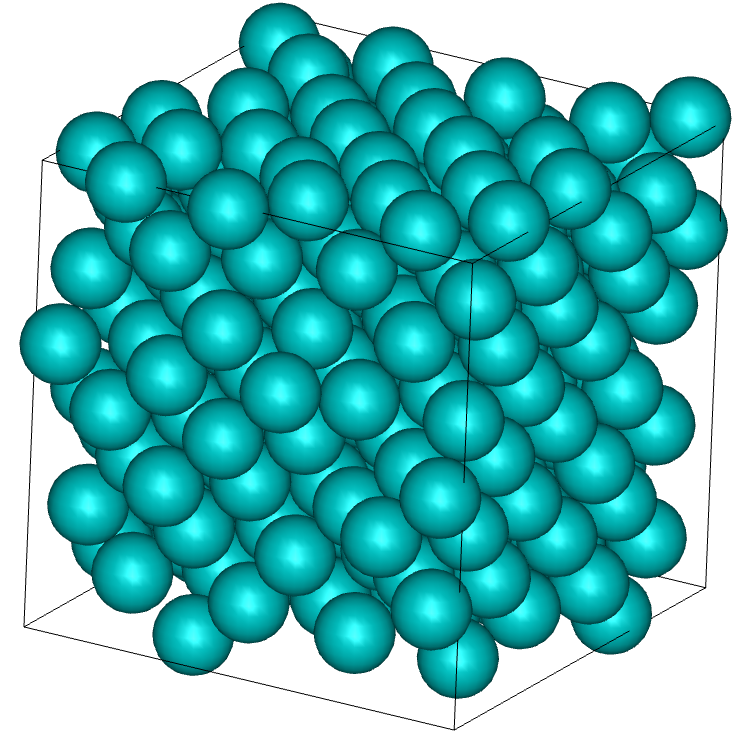
\includegraphics[width=0.6\linewidth]{graphs/P2E2/coords_1.15.png}
	\caption{Final coordinates for an FCC lattice with a density of $\rho \sigma^3 = 1.15$.}
	\label{fig: coords 1.15}
\end{figure}
\newpage
\subsection{MD MSD for $\bf{\rho \sigma^3 = 0.01}$ and 0.6}
We can straightforwardly change our MD simulation of the previous exercise with the  Lennerd-Jones to the WCA potential by changing the $r_{cut}$ form $2.5 \sigma$ to $2^{\frac{1}{6}} \sigma$. 
We than get the following MSD for $\rho \sigma^3$ = 0.01 and 0.6 respectively.


\begin{figure}[H]
	\centering
	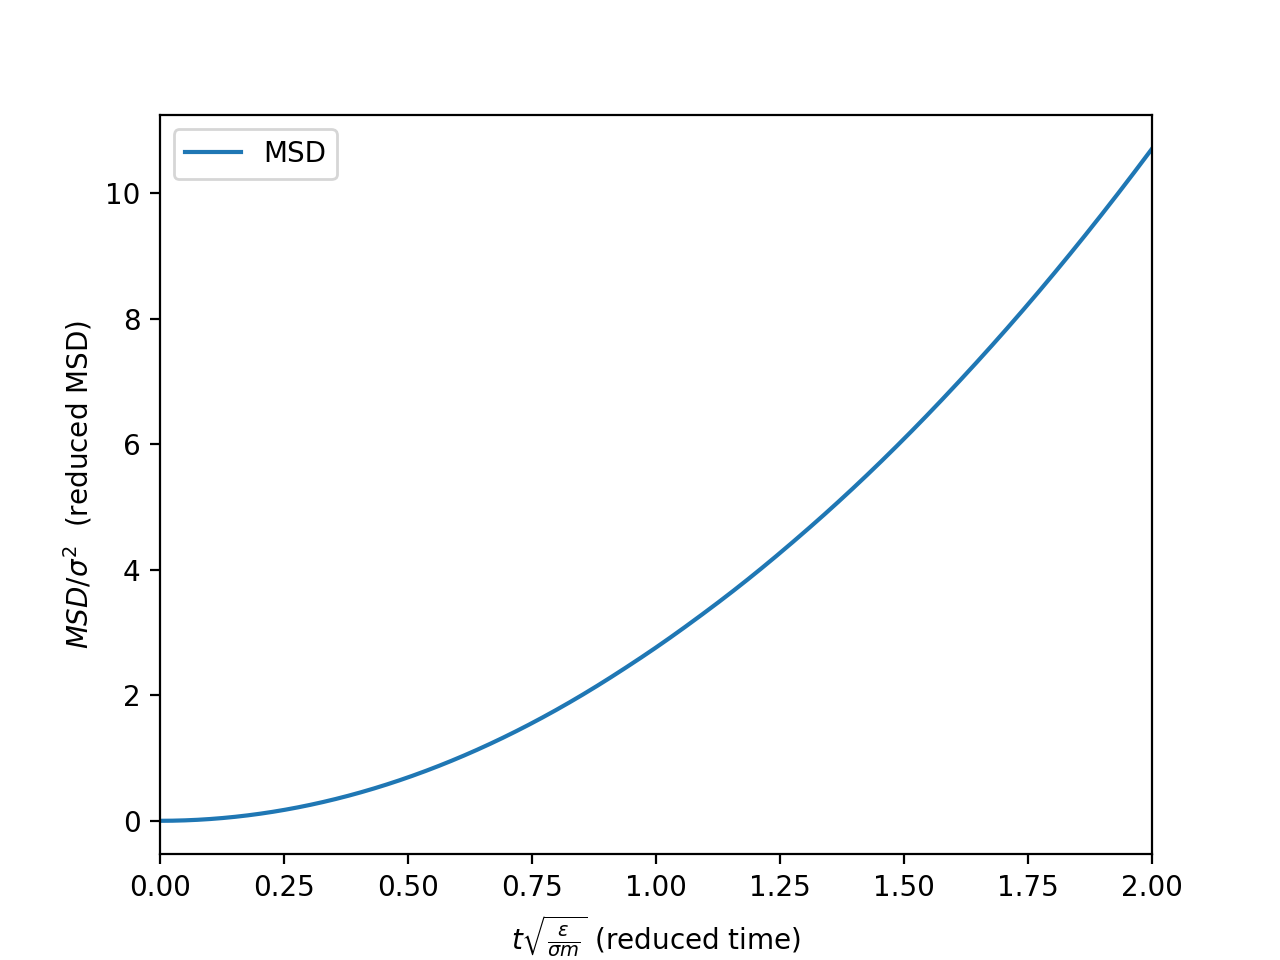
\includegraphics[width=0.75\linewidth]{graphs/P2E2/MD_MSD_001.png}
	\caption{MSD for an MD simulation with a WCA potential at a density of $\rho \sigma^3 = 0.01$.}
	\label{fig: MSD MD 0.01}
\end{figure}

\begin{figure}[H]
	\centering
	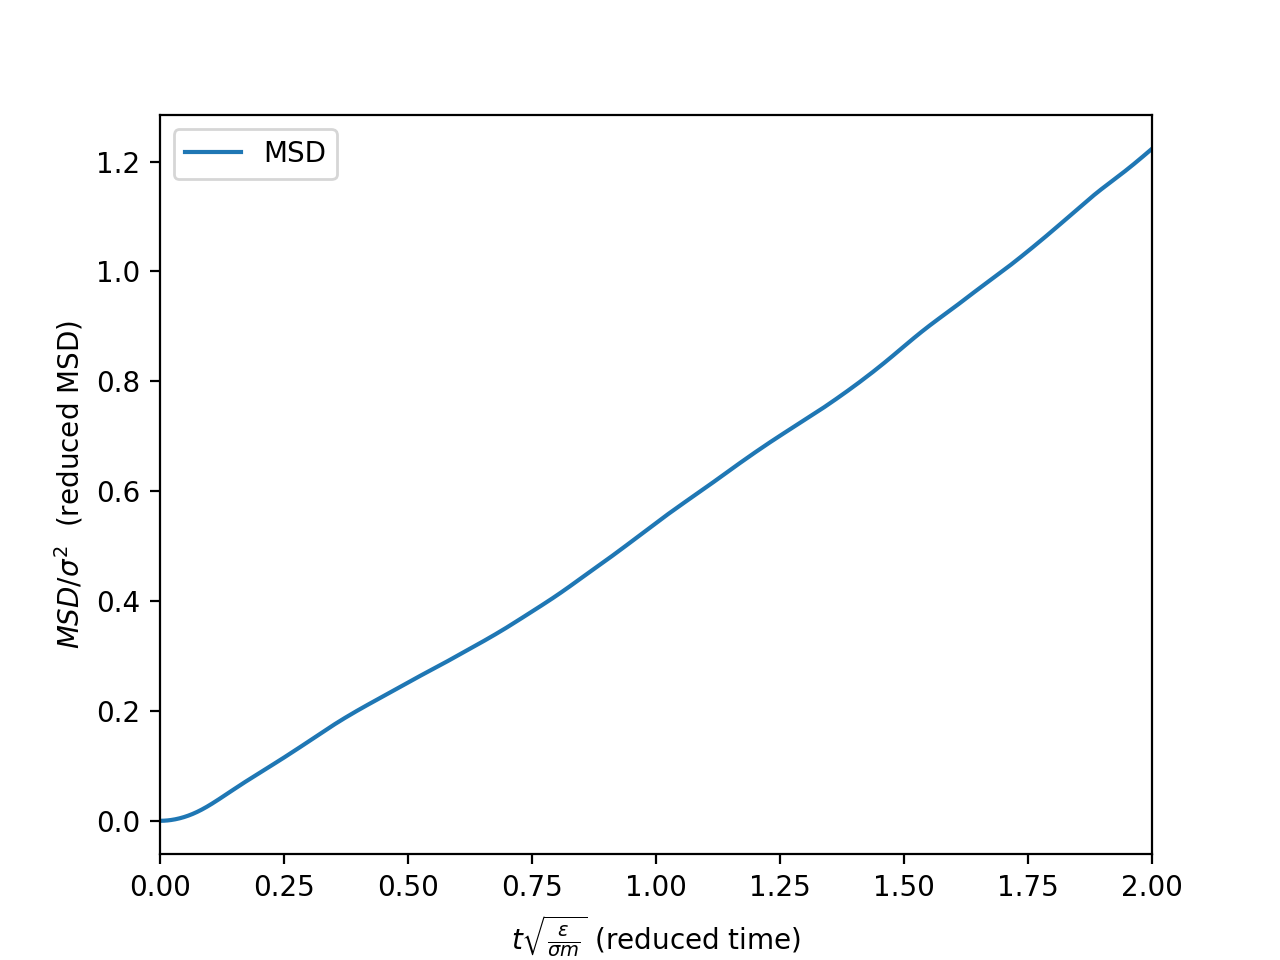
\includegraphics[width=0.75\linewidth]{graphs/P2E2/MD_MSD_06.png}
	\caption{MSD for an MD simulation with a WCA potential at a density of $\rho \sigma^3 = 0.6$.}
	\label{fig: MSD MD 0.6}
\end{figure}

When comparing the MSD of the MD simulation to the BM simulation there are a couple of distinct differences.
Firstly the MD simulation has a smooth result unlike the BM which is logical since the MD simulation does not use the random force of the BM.
Secondly we see that the MD has a lower MSD than the BM with a larger difference for the density of 0.6 than for 0.01. 
Lastly we do not see the clear linear model for the MD simulation that we did see in the BM simulation where the 0.01 case in particular seems to be increasing on the entire time frame and seems to be in the ballistic regime.
We start of with the initial velocity from our Boltzman distribution and because of the low density the displacement is linear. This means that with a linear displacement the squared displacement is quadratic.
The higher density seems to be more linear but is not linear when we try to fit it.

\begin{figure}[H]
	\centering
	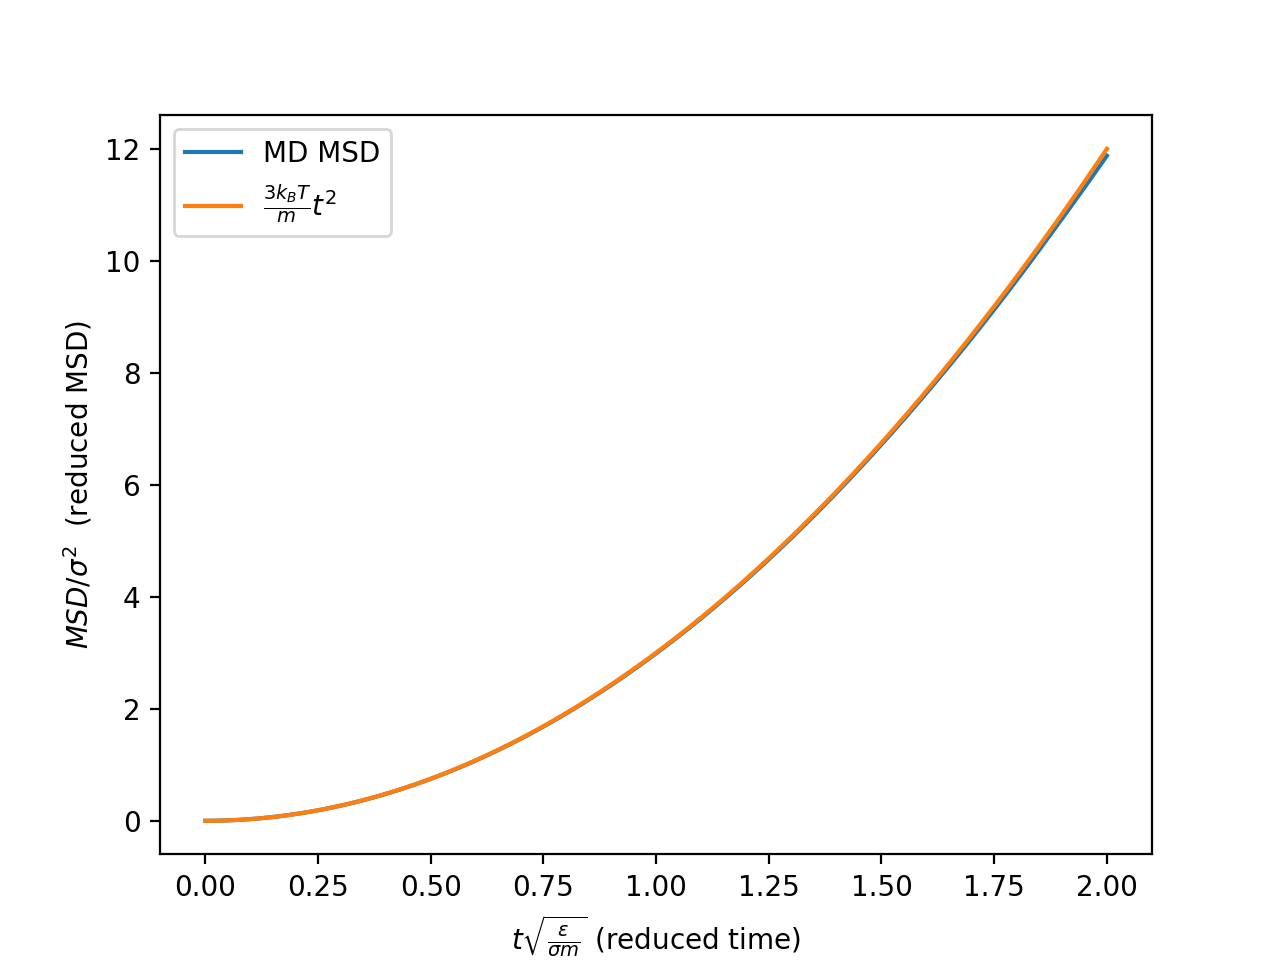
\includegraphics[width=0.75\linewidth]{graphs/P2E2/MD_MSD_06-fit.png}
	\caption{MSD for an MD simulation with a WCA potential at a density of $\rho \sigma^3 = 0.01$ and the theoretical model in the ballistic regime where we see a perfect match.}
	\label{fig: MSD MD 0.6}
\end{figure}
